\documentclass[]{article}
\usepackage{lmodern}
\usepackage{amssymb,amsmath}
\usepackage{ifxetex,ifluatex}
\usepackage{fixltx2e} % provides \textsubscript
\ifnum 0\ifxetex 1\fi\ifluatex 1\fi=0 % if pdftex
  \usepackage[T1]{fontenc}
  \usepackage[utf8]{inputenc}
\else % if luatex or xelatex
  \ifxetex
    \usepackage{mathspec}
  \else
    \usepackage{fontspec}
  \fi
  \defaultfontfeatures{Ligatures=TeX,Scale=MatchLowercase}
\fi
% use upquote if available, for straight quotes in verbatim environments
\IfFileExists{upquote.sty}{\usepackage{upquote}}{}
% use microtype if available
\IfFileExists{microtype.sty}{%
\usepackage[]{microtype}
\UseMicrotypeSet[protrusion]{basicmath} % disable protrusion for tt fonts
}{}
\PassOptionsToPackage{hyphens}{url} % url is loaded by hyperref
\usepackage[unicode=true]{hyperref}
\hypersetup{
            pdfborder={0 0 0},
            breaklinks=true}
\urlstyle{same}  % don't use monospace font for urls
\usepackage{graphicx,grffile}
\makeatletter
\def\maxwidth{\ifdim\Gin@nat@width>\linewidth\linewidth\else\Gin@nat@width\fi}
\def\maxheight{\ifdim\Gin@nat@height>\textheight\textheight\else\Gin@nat@height\fi}
\makeatother
% Scale images if necessary, so that they will not overflow the page
% margins by default, and it is still possible to overwrite the defaults
% using explicit options in \includegraphics[width, height, ...]{}
\setkeys{Gin}{width=\maxwidth,height=\maxheight,keepaspectratio}
\IfFileExists{parskip.sty}{%
\usepackage{parskip}
}{% else
\setlength{\parindent}{0pt}
\setlength{\parskip}{6pt plus 2pt minus 1pt}
}
\setlength{\emergencystretch}{3em}  % prevent overfull lines
\providecommand{\tightlist}{%
  \setlength{\itemsep}{0pt}\setlength{\parskip}{0pt}}
\setcounter{secnumdepth}{0}
% Redefines (sub)paragraphs to behave more like sections
\ifx\paragraph\undefined\else
\let\oldparagraph\paragraph
\renewcommand{\paragraph}[1]{\oldparagraph{#1}\mbox{}}
\fi
\ifx\subparagraph\undefined\else
\let\oldsubparagraph\subparagraph
\renewcommand{\subparagraph}[1]{\oldsubparagraph{#1}\mbox{}}
\fi

% set default figure placement to htbp
\makeatletter
\def\fps@figure{htbp}
\makeatother


\date{}

\begin{document}

\begin{quote}
\textbf{Работа 3.4.2}

Закон Кюри---Вейсса

\textbf{Цель работы:} изучение температурной зависимости магнитной
вос­приимчивости ферромагнетика выше точки Кюри.

\textbf{В работе используются:} катушка самоиндукции с образ­цом из
гадолиния, термостат, частотомер, цифровой вольтметр, LC-автогенератор,
термопара медь-константан.
\end{quote}

Вещества с отличными от нуля атомными магнитными моментами обладают
парамагнитными свойствами. Внешнее магнитное поле ориен­тирует магнитные
момент, которые в отсутствие поля располагались в пространстве хаотичным
образом.

\begin{quote}
При повышении температуры \emph{Т} возрастает дезориентирующее дей­ствие
теплового движения частиц, и магнитная восприимчивость па­рамагнетиков
убывает, в простейшем случае (в постоянном магнитном поле) --- по закону
Кюри:
\end{quote}

\textbf{(1)}

\begin{quote}
где \emph{С ---} постоянная Кюри.

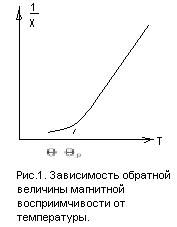
\includegraphics[width=1.84306in,height=2.37153in]{./media/image2.png}

Для парамагнитных веществ, которые при понижении температуры становятся
ферромагнитными, формула (1) должна быть видоизмене­на. Эта формула
показывает, что температура \emph{Т =} 0 является особой точкой
температурной кривой, в которой \emph{х} неограниченно возрастает. При
\emph{Т} ---\emph{\textgreater{}} 0 тепловое движение всё меньше
препятствует магнитным моментам атомов ори­ентироваться в одном
направлении при сколь угодно слабом внешнем поле. В ферромагнети­ках ---
под влиянием обменных сил --- это про­исходит при понижении температуры
не до абсо­лютного нуля, а до температуры Кюри θ. Для ферромагнетиков
закон Кюри дол­жен быть заменён законом Кюри-Вейсса:
\end{quote}

χ\textasciitilde{} (1)

\begin{quote}
где \emph{θр ---} температура, близкая к температуре Кюри.

Эта формула хорошо описывает поведение ферромагнитных ве­ществ после их
перехода в парамагнитную фазу при заметном удалении температуры от θ, но
недостаточно точна при \emph{Т} \textasciitilde{}θ .

Иногда для уточнения формулы (2) вводят вместо одной две темпе­ратуры
Кюри, одна из которых описывает точку фазового перехода ---
ферромагнитная точка Кюри θ, а другая является параметром в фор­муле (2)
--- парамагнитная точка Кюри --- \emph{θ\textsubscript{р}} (рис. 1).

В нашей работе изучается температурная зависимость χ(T) гадоли­ния при
температурах выше точки Кюри. Выбор материала определяет­ся тем, что его
точка Кюри лежит в интервале комнатных температур.
\end{quote}

\textbf{Экспериментальная установка}. Схема установки для проверки
за­кона Кюри---Вейсса показана на рис. 2. Исследуемый ферромагнитный
образец (гадолиний) расположен внутри пустотелой катушки самоин­дукции,
которая служит индуктивностью колебательного контура, вхо­дящего в
состав LC-автогенератора. Автогенератор собран на полевом транзисторе
КП-103 и смонтирован в виде отдельного блока.
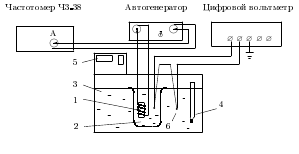
\includegraphics[width=3.11458in,height=1.61458in]{./media/image5.png}

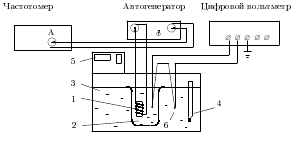
\includegraphics[width=3.10000in,height=1.48542in]{./media/image6.png}

Рис. 2. Схема экспериментальной установки

Гадолиний является хорошим проводником электрического тока, а рабочая
частота генератора достаточно велика (\textasciitilde{}50 кГц), поэтому
для уменьшения вихревых токов образец изготовлен из мелких кусочков
размером около . Катушка 1 с образцом помещена в стеклянный сосуд 2,
залитый трансформаторным маслом. Масло предохраняет об­разец от
окисления и способствует ухудшению электрического контак­та между
отдельными частичками образца. Кроме того, оно улучшает тепловой контакт
между образцом и термостатируемой (рабочей) жид­костью 3 в термостате.
Ртутный термометр 4 используется для прибли­жённой оценки температуры.
Температура образца регулируется с по­мощью термостата.

Магнитная восприимчивость образца \emph{χ} определяется по изменению
самоиндукции катушки. Следует отметить,что восприимчивость образца
отличается от восприимчивости гадолиния из-за достаточно большого
размагничивающего коэффициента. Обозначив через \emph{L} самоиндукцию
катушки с образцом и через \emph{\textsc{L\textsubscript{0}} ---} её
самоиндукцию в отсутствие образца, по­лучим

\begin{quote}
\emph{(L --} L\textsubscript{0}) \textasciitilde{} χ (3)
\end{quote}

При изменении самоиндукции образца меняется период колебаний
ав­тогенератора:

\begin{quote}
\emph{\textsc{,}} (4)
\end{quote}

где \emph{С ---} ёмкость контура автогенератора.

Период колебаний в отсутствие образца определяется самоиндукци­ей пустой
катушки:

\begin{quote}
\emph{.} (5)

Из (4) и (5) имеем

(L\emph{-L\textsubscript{0})\textasciitilde{}}
\end{quote}

Таким образом,

\textbf{\textasciitilde{} (6)}

\begin{quote}
Из формул (2) и (6) следует, что закон Кюри-Вейсса справедлив, если
выполнено соотношение
\end{quote}

\textbf{(7)}

χ\textasciitilde{}(T-θ\textsubscript{p})\textasciitilde{}

\begin{quote}
Измерения проводятся в интервале температур от 14 °С до 40 °С. С целью
экономии времени следует начинать измерения с низких тем­ператур.
\end{quote}

Для охлаждения образца используется холодная водопроводная во­да,
циркулирующая вокруг сосуда с рабочей жидкостью (дистиллиро­ванной
водой); рабочая жидкость постоянно перемешивается.

\begin{quote}
Величина стабилизируемой температуры задаётся на дисплее 5 тер­мостата.
Для нагрева служит внутренний электронагреватель, не по­казанный на
рисунке. Когда температура рабочей жидкости в сосуде приближается к
заданной, непрерывный режим работы нагревателя ав­томатически переходит
в импульсный (нагреватель то включается, то выключается) --- начинается
процесс стабилизации температуры.

Измерения проводятся в интервале температур от 14 °С до 40 °С. С целью
экономии времени следует начинать измерения с низких тем­ператур.
\end{quote}

Для охлаждения образца используется холодная водопроводная во­да,
циркулирующая вокруг сосуда с рабочей жидкостью (дистиллиро­ванной
водой); рабочая жидкость постоянно перемешивается.

\begin{quote}
Величина стабилизируемой температуры задаётся на дисплее 5 тер­мостата.
Для нагрева служит внутренний электронагреватель, не по­казанный на
рисунке. Когда температура рабочей жидкости в сосуде приближается к
заданной, непрерывный режим работы нагревателя ав­томатически переходит
в импульсный (нагреватель то включается, то выключается) --- начинается
процесс стабилизации температуры.
\end{quote}

Температура исследуемого образца всегда несколько отличается от
температуры дистиллированной воды в сосуде. После того как вода
до­стигла заданной температуры, идёт медленный процесс выравнивания
температур образца и воды. Разность их температур контролируется с
помощью медно-константановой термопары 6 и цифрового вольтметра. Один из
спаев термопары находится в тепловом контакте с образцом, а другой
погружён в воду. Концы термопары подключены к цифровому вольтметру.
Чувствительность термопары указана на установке. Реко­мендуется измерять
период колебаний автогенератора в тот момент, когда указанная разность
температур становится меньше 0,5 °С (более точному измерению температур
мешают паразитные ЭДС, возникаю­щие в цепи термопары).

\begin{quote}
ЗАДАНИЕ

В работе предлагается исследовать зависимость периода колебаний
автогенератора от температуры сердечника катушки и по результатам
измерений определить парамагнитную точку Кюри гадолиния.
\end{quote}

\begin{enumerate}
\def\labelenumi{\arabic{enumi}.}
\item
  \begin{quote}
  Подготовьте приборы к работе.
  \end{quote}
\end{enumerate}

\begin{quote}
Оцените допустимую ЭДС термопары, если допустимая разность тем­ператур
образца и рабочей жидкости \emph{ΔT =} 0,5 °С, а постоянная термо­пары
\emph{к =} 24 град/мВ;

2. Исследуйте зависимость периода колебаний LC-генератора от
темпе­ратуры образца, отмечая период колебаний \emph{τ} по частотомеру,
а тем­пературу \emph{Т} --- по показаниям дисплея и цифровому вольтметру
(ΔUс учётом знака). Термопара подключена так, что при знаке «+» на
таб­ло вольтметра температура образца выше температуры рабочей
жид­кости.

Проведите измерения в диапазоне от 14 °С до 40 °С через 2°С. Запишите
период колебаний τ\textsubscript{0} без образца, указанный на установке.

3. Закончив измерения, охладите термостат, руководствуясь техниче­ским
описанием.
\end{quote}

Обработка результатов

\begin{enumerate}
\def\labelenumi{\arabic{enumi}.}
\item
  \begin{quote}
  Рассчитайте температуру \emph{Т} образца с учётом показаний
  термопары.\\
  Постройте график зависимости
  1/(τ\textsuperscript{2}-τ\textsubscript{0}\textsuperscript{2})=
  \emph{f(T).} Экстраполируя
  \end{quote}
\end{enumerate}

по­лученную прямую к оси абсцисс, определите парамагнитную точку Кю­ри
\emph{θ\textsubscript{р}} для гадолиния.

\begin{enumerate}
\def\labelenumi{\arabic{enumi}.}
\item
  \begin{quote}
  Оцените погрешности эксперимента и сравните результат с табличным.
  \end{quote}
\end{enumerate}

\begin{quote}
\textbf{Контрольные вопросы}
\end{quote}

\begin{enumerate}
\def\labelenumi{\arabic{enumi}.}
\item
  \begin{quote}
  Как объяснить явления пара- и диамагнетизма с молекулярной точки
  зре­ния?
  \end{quote}
\item
  \begin{quote}
  Чем отличаются пара- и ферромагнетики в отсутствие магнитного поля?
  \end{quote}
\item
  \begin{quote}
  Сформулируйте общий физический принцип, объясняющий явление
  диа­магнетизма.
  \end{quote}
\item
  \begin{quote}
  Качественно изобразите на одном графике \emph{В(Н)} для пара-, диа- и
  ферро­магнетика.
  \end{quote}
\end{enumerate}

5* Какой вклад в магнитную восприимчивость образца вносит проводимость
гадолиния? Как связан этот вклад с размером крупинок, частотой и
удельной проводимостью? Зависит ли этот вклад от температуры? Оцените
этот вклад для крупинок размером . Обратите внимание на рис.1, на
котором кривая около точки Кюри идёт практически горизонтально, не
опускаясь до нуля. Оцените глубину проникания магнитного поля около
точки Кюри, считая магнитную проницаемость и проводимость примерно
такими же, как у железа.

\begin{quote}
СПИСОК ЛИТЕРАТУРЫ
\end{quote}

\begin{enumerate}
\def\labelenumi{\arabic{enumi}.}
\item
  \begin{quote}
  \emph{Сивухин Д-В.} Общий курс физики. Т. III. Электричество. --- М.:
  Наука,\\
  1983. §§ 74, 79.
  \end{quote}
\item
  \begin{quote}
  \emph{Калашников С.Г.} Электричество. --- М.: Наука, 1977. §§ 110,
  111, 119.
  \end{quote}
\end{enumerate}

\end{document}
